\documentclass[12pt]{article}  
%%Read the manual for other options. 

\pagestyle{empty} %%Eliminates page numbers
%%\input rmb_macros
%%Collect your favorite macros in a 
%%separate file

%\input amssym.def
%\input amssym
%\input mssymb
%%Defines additional symbols



\usepackage{graphics}
\usepackage{amsmath,amssymb,amsthm, multicol}
\usepackage[pdftex]{graphicx}
\usepackage{epsf}
%%Use to include pictures. 

%\newcommand{\comment}[1]{}
%\newcommand{\sobolev}[2]{W^{#1,#2}}
%\newcommand{\sobolev}[2]{L^#2_#1}
%%Some examples of macros or new commands.

\addtolength{\oddsidemargin}{-.75in}
\addtolength{\evensidemargin}{-.75in}
\addtolength{\textwidth}{1.5in}
\addtolength{\topmargin}{-1in}
\addtolength{\textheight}{2.25in}
%%Set margins, defaults are ok. 

\begin{document}
\begin{flushleft} 
%%Paragraphs will not be indented in this 
%%environment
\centerline{\LARGE{Quiz 3}} 
\vspace{5 mm}
{Student ID Number:}\hfill  
%%\hfill forces following text 
%%to right margin
{Name \rule {2 in}{0.01in}}\\
Math 173B, 1PM
\\
%%gives a line of length 2in and 
%%thickness 0.01in
{Please justify all your answers}\hfill {January 24, 2019}
\\
{Please also write your full name on the back} 

\medskip
\end{flushleft}

\begin{enumerate}
	\item Below is a Vigen\`ere ciphertext in which some of the repeated trigrams have been underlined. How long do you think the keyword is? Why?

	\begin{figure}[h]
	\centering
		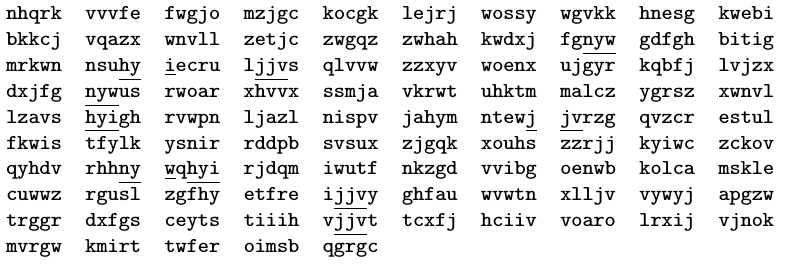
\includegraphics[scale=.5]{vig.png}
	\end{figure}
	\vfill

	\item Your friend offers you a bet. You roll two six-sided dice. You win \$100 if their sum is five and lose \$12 otherwise. Do you take this bet? How much money do you expect to win or lose if you were to take this bet 25 times?

	\vfill
\end{enumerate}

%\vfill will divide page evenly
%use \begin{enumerate} environment for ordered lists
\end{document}